\documentclass[10pt,a4paper]{article}

% ---------------------------------------------------------------------------- %
% PACKAGES
% ---------------------------------------------------------------------------- %

\usepackage[
    top=1.8cm,
    bottom=1.8cm,
    left=1.7cm,
    right=1.7cm
]{geometry}

\usepackage{fontspec}
\usepackage{xcolor}
\usepackage{titlesec}
\usepackage{tocloft}
\usepackage{amssymb}
\usepackage{mathtools}
\usepackage{amsthm}
\usepackage{graphicx} 
\usepackage{listings}
\usepackage{fancyhdr}
\usepackage{microtype}
\usepackage{hyperref}

\numberwithin{equation}{section}

% ---------------------------------------------------------------------------- %
% DOCUMENT
% ---------------------------------------------------------------------------- %

\pagestyle{fancy}
\fancyhf{}
\fancyhead[L]{\small\DocumentTitle}
\fancyhead[R]{\small\nouppercase{\leftmark}}
\fancyfoot[C]{\thepage}
\setlength{\headheight}{14pt}

% ---------------------------------------------------------------------------- %
% FONT
% ---------------------------------------------------------------------------- %

\newcommand{\TextFont}{TeX Gyre Heros}
\newcommand{\HeaderFont}{TeX Gyre Adventor}

\setmainfont{\TextFont}
\newfontfamily\HeaderFamily{\HeaderFont}

% ---------------------------------------------------------------------------- %
% COLOURS
% ---------------------------------------------------------------------------- %

\definecolor{Black}{HTML}{000000}
\definecolor{DarkGrey}{HTML}{333333}
\definecolor{Grey}{HTML}{666666}
\definecolor{LightGrey}{HTML}{CCCCCC}

% ---------------------------------------------------------------------------- %
% FONT SIZE
% ---------------------------------------------------------------------------- %

\newcommand{\TitleSize}{32}
\newcommand{\SubtitleSize}{16}

\newcommand{\HeaderOneSize}{22}
\newcommand{\HeaderTwoSize}{16}
\newcommand{\HeaderThreeSize}{12}

\newcommand{\TextSize}{10}

% ---------------------------------------------------------------------------- %
% LINE SPACING
% ---------------------------------------------------------------------------- %

\newcommand{\TitleSpacing}{38}
\newcommand{\SubtitleSpacing}{20}

\newcommand{\HeaderOneSpacing}{26}
\newcommand{\HeaderTwoSpacing}{20}
\newcommand{\HeaderThreeSpacing}{16}

% ---------------------------------------------------------------------------- %
% SECTION FORMAT
% ---------------------------------------------------------------------------- %

\titleformat
    {\section}
    {\HeaderFamily\fontsize{\HeaderOneSize}{\HeaderOneSpacing}\selectfont\bfseries}
    {\thesection}
    {0.75em}
    {}

\titlespacing*{\section}
    {0pt}
    {1.5cm}
    {0.5cm}

% ---------------------------------------------------------------------------- %
% SUBSECTION FORMAT
% ---------------------------------------------------------------------------- %

\titleformat
    {\subsection}
    {\HeaderFamily\fontsize{\HeaderTwoSize}{\HeaderTwoSpacing}\selectfont\bfseries}
    {\thesubsection}
    {0.75em}
    {}

\titlespacing*{\subsection}
    {0pt}
    {0.8cm}
    {0.3cm}

% ---------------------------------------------------------------------------- %
% SUBSUBSECTION FORMAT
% ---------------------------------------------------------------------------- %

\titleformat
    {\subsubsection}
    {\HeaderFamily\fontsize{\HeaderThreeSize}{\HeaderThreeSpacing}\selectfont\bfseries}
    {\thesubsubsection}
    {0.75em}
    {}

\titlespacing*{\subsubsection}
    {0pt}
    {0.6cm}
    {0.2cm}

% ---------------------------------------------------------------------------- %
% TABLE OF CONTENTS
% ---------------------------------------------------------------------------- %

\renewcommand{\cftsecfont}{\bfseries}
\renewcommand{\cftsecpagefont}{\bfseries}

\setlength{\cftbeforesecskip}{0.4em}

% ---------------------------------------------------------------------------- %
% HYPERLINKS
% ---------------------------------------------------------------------------- %

\hypersetup{
    colorlinks=true,
    linkcolor=Black,
    urlcolor=Grey,
    citecolor=Black
}

% ---------------------------------------------------------------------------- %
% DOCUMENT INFORMATION
% ---------------------------------------------------------------------------- %

\newcommand{\DocumentTitle}{Lie Groups and Lie Algebras for Robotics}
\newcommand{\DocumentSubtitle}{Rotations and Rigid-Body Transformations}
\newcommand{\DocumentAuthor}{Jason Wakim Richards}
\newcommand{\DocumentDate}{\today}

% ---------------------------------------------------------------------------- %
% TITLE PAGE
% ---------------------------------------------------------------------------- %

\newcommand{\TitlePage}{
    \begin{titlepage}

        \vspace*{3cm}

        {\HeaderFamily
        \fontsize{\TitleSize}{\TitleSpacing}
        \selectfont
        \bfseries
        \DocumentTitle\par}

        \vspace{0.5cm}

        {\fontsize{\SubtitleSize}{\SubtitleSpacing}
        \selectfont
        \DocumentSubtitle\par}

        \vspace{1cm}

        \noindent
        \textcolor{LightGrey}{\rule{\textwidth}{1pt}}

        \vfill

        {\fontsize{12}{16}\selectfont
        \DocumentAuthor\par}

        \vspace{0.2cm}

        {\fontsize{10}{14}\selectfont
        \DocumentDate\par}

    \end{titlepage}
}

% ---------------------------------------------------------------------------- %
% SECTION COMMANDS
% ---------------------------------------------------------------------------- %

\newcommand{\Section}[1]{\section{#1}}
\newcommand{\Subsection}[1]{\subsection{#1}}
\newcommand{\Subsubsection}[1]{\subsubsection{#1}}
\newcommand{\Property}[1]{\par\noindent\textbf{#1}\par}

\newcommand{\SOthree}{\mathrm{SO}(3)}
\newcommand{\SEthree}{\mathrm{SE}(3)}
\newcommand{\sothree}{\mathfrak{so}(3)}
\newcommand{\sethree}{\mathfrak{se}(3)}
\newcommand{\Exp}{\operatorname{Exp}}
\newcommand{\Log}{\operatorname{Log}}
\newcommand{\tr}{\operatorname{tr}}
\newcommand{\vect}[1]{\boldsymbol{#1}}

\theoremstyle{definition}
\newtheorem{definition}{Definition}[section]
\newtheorem{example}{Example}[section]
\newtheoremstyle{exercisestyle}
    {1.2em}
    {1.2em}
    {\normalfont}
    {0pt}
    {\bfseries\color{DarkGrey}}
    {.}
    {\newline}
    {}
\theoremstyle{exercisestyle}
\newtheorem{exercise}{Exercise}[section]

\newenvironment{tasks}
    {\par\begin{quote}\small\textbf{Tasks}\par\smallskip}
    {\end{quote}}

\lstset{
    basicstyle=\ttfamily\small,
    frame=single,
    columns=fullflexible,
    keepspaces=true,
    showstringspaces=false
}

% ---------------------------------------------------------------------------- %
% DOCUMENT
% ---------------------------------------------------------------------------- %

\setlength{\parindent}{0pt}
\setlength{\parskip}{0.6em}

\begin{document}

\hypersetup{pageanchor=false}
\TitlePage
\hypersetup{pageanchor=true}
\pagenumbering{roman}

\tableofcontents

\newpage
\pagenumbering{arabic}

\Section{Introduction}

This document introduces the Lie groups used to represent three-dimensional
rotations and rigid-body transformations in robotics. It develops the geometry
of $\SOthree$ and $\SEthree$, their Lie algebras, and the exponential and
logarithmic maps that connect them. Worked examples and implementation notes
show how these ideas are used in estimation, control, computer vision, and
simultaneous localisation and mapping (SLAM).

The reader should be comfortable with vectors, matrices, matrix multiplication,
determinants, and basic calculus. By the end of the document, the reader should
be able to:

\begin{itemize}
    \item interpret frame-labelled rotations and transformations;
    \item distinguish a Lie group element from its Lie algebra coordinates;
    \item compute and interpret the exponential and logarithmic maps of
          $\SOthree$ and $\SEthree$;
    \item compose and invert rigid-body transformations; and
    \item distinguish active and passive transformations from left and right
          perturbations.
\end{itemize}

\Subsection{Notation and conventions}

Vectors are bold lowercase symbols, matrices are bold uppercase symbols, and
all coordinate frames are right-handed. The notation ${}^B\mathbf{R}_A$ denotes
the rotation that maps vector coordinates from frame $A$ to frame $B$.
Similarly, ${}^B\mathbf{T}_A$ maps homogeneous point coordinates from frame $A$
to frame $B$. Angles are measured in radians.

The groups are written $\SOthree$ and $\SEthree$, while their Lie algebras are
written $\sothree$ and $\sethree$. The hat operator $(\cdot)^\wedge$ maps vector
coordinates to a Lie algebra matrix; the vee operator $(\cdot)^\vee$ is its
inverse. This document uses $\Exp$ and $\Log$ for vector-valued Lie-group maps
and $\exp$ and $\log$ for matrix functions.

\Section{Coordinate Frames}

Consider two coordinate frames, $A$ and $B$. Let
${}^B\mathbf{R}_A \in \SOthree$ map vector coordinates from frame $A$ to frame
$B$, and let ${}^B\mathbf{t}_A \in \mathbb{R}^3$ be the position of the origin
of frame $A$, measured from the origin of frame $B$ and expressed in frame $B$.
A point with coordinates ${}^A\mathbf{p}$ in frame $A$ has coordinates
${}^B\mathbf{p}$ in frame $B$ given by

\begin{equation}
    {}^B\mathbf{p}
    =
    {}^B\mathbf{R}_A {}^A\mathbf{p}
    +
    {}^B\mathbf{t}_A
    \label{eq:point-transformation}
\end{equation}

This coordinate transformation contains both a rotation and a translation. The
quantities in \eqref{eq:point-transformation} are:

\vspace{0.5cm}

\renewcommand{\arraystretch}{1.6}
\begin{tabular}{@{}ll}
    ${}^B\mathbf{p}$   & point expressed in frame $B$;                       \\
    ${}^B\mathbf{R}_A$ & coordinate rotation from frame $A$ to frame $B$;    \\
    ${}^A\mathbf{p}$   & point expressed in frame $A$;                       \\
    ${}^B\mathbf{t}_A$ & position of the $A$-origin, expressed in frame $B$.
\end{tabular}

\vspace{0.5cm}

It is important to get a clear understanding of what the variables mean and what
frames they are in. Figure \ref{fig:coordinate-frames} shows a diagram of the
different vectors.

\vspace{0.3cm}

\begin{figure}[ht]
    \centering
    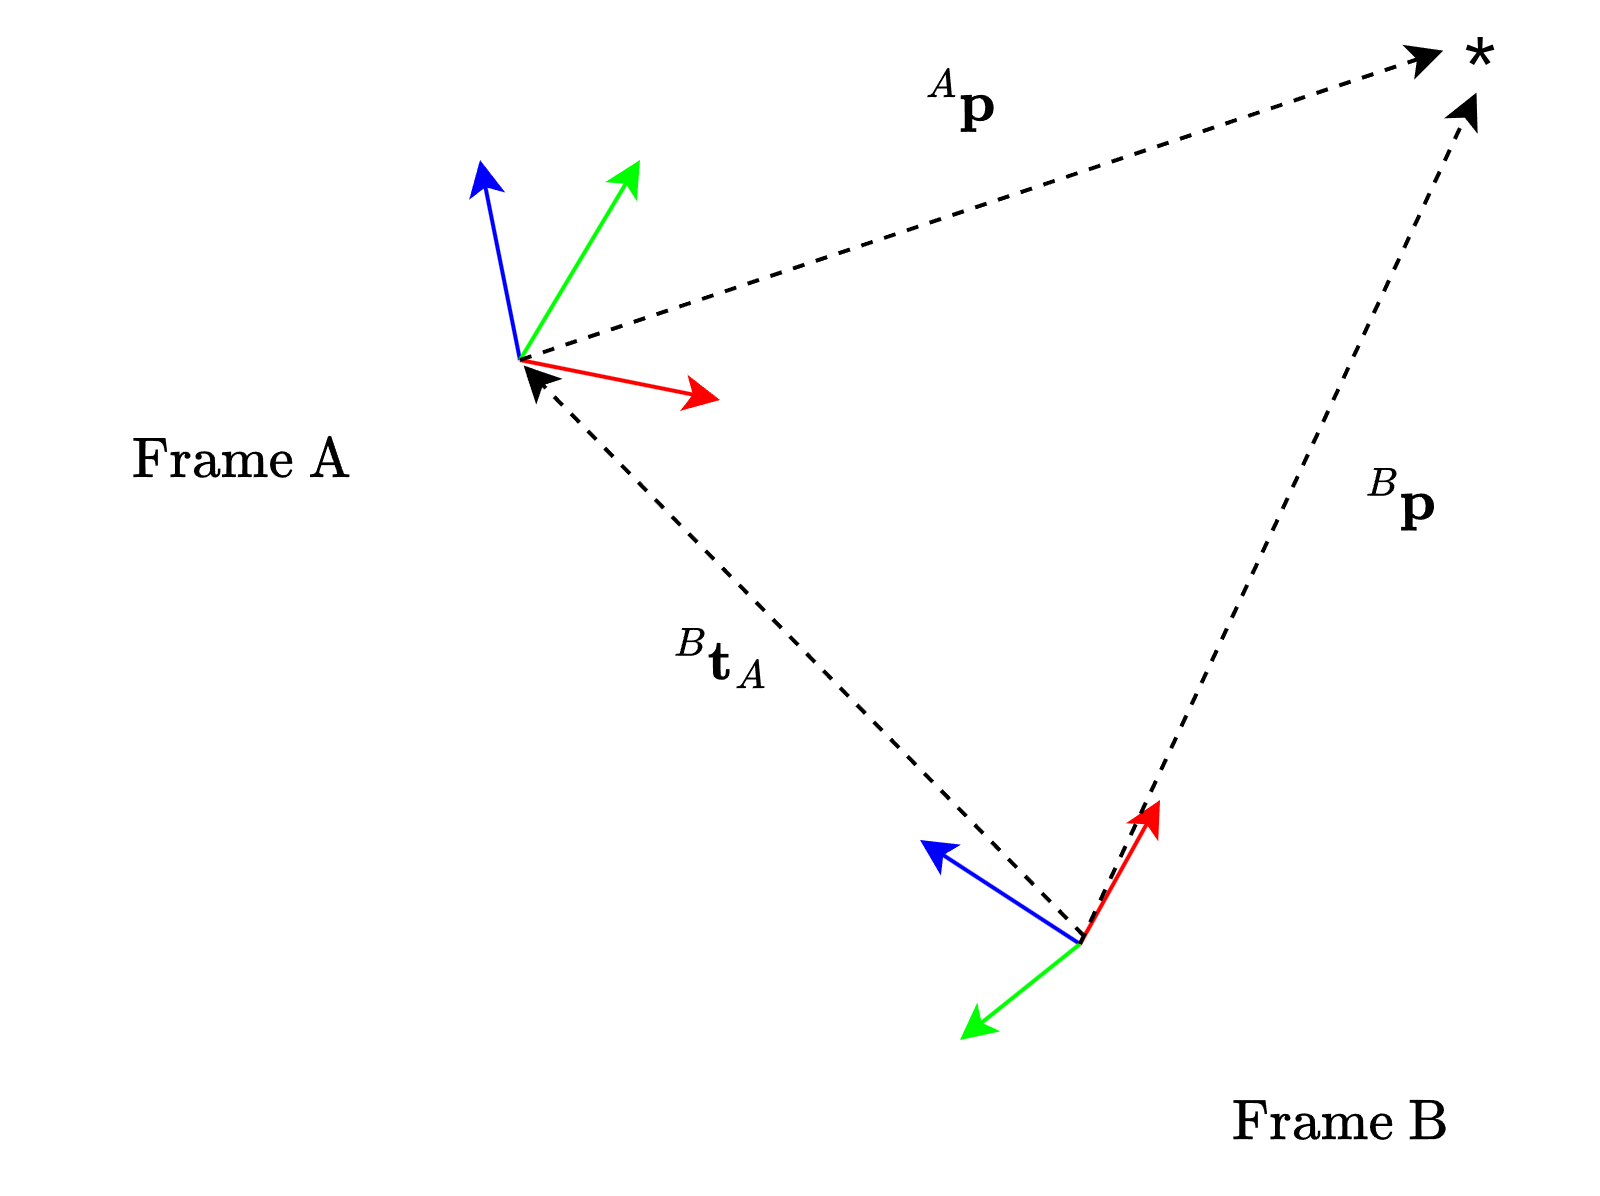
\includegraphics[width=0.7\textwidth]{figures/png/robotics-exercises-lie-group-algebra.png}
    \caption{The same geometric point expressed in frames $A$ and $B$. The
        translation ${}^B\mathbf{t}_A$ points from the $B$-origin to the $A$-origin
        and is expressed in frame $B$.}
    \label{fig:coordinate-frames}
\end{figure}

\Section{SO(3): Rotations}

A point is represented by a vector in $\mathbb{R}^3$; a rotation of that point
is represented by a matrix

\begin{equation}
    \mathbf{R} = \begin{bmatrix}
        r_{11} & r_{12} & r_{13} \\
        r_{21} & r_{22} & r_{23} \\
        r_{31} & r_{32} & r_{33}
    \end{bmatrix}.
    \label{eq:rotation-matrix}
\end{equation}

\begin{definition}
    The special orthogonal group in three dimensions is
    \begin{equation}
        \SOthree =
        \left\{\mathbf{R}\in\mathbb{R}^{3\times3}
        \;\middle|\;
        \mathbf{R}^{\mathsf T}\mathbf{R}=\mathbf{I}_3,
        \ \det(\mathbf{R})=1\right\}.
        \label{eq:so3-definition}
    \end{equation}
    Its elements are the proper rotation matrices.
\end{definition}

Orthogonality implies
$\mathbf{R}^{-1}=\mathbf{R}^{\mathsf T}$. The determinant constraint excludes
reflections. Although a general $3\times3$ matrix has nine entries, these
constraints leave only three degrees of freedom.

\Subsection{Why is SO(3) a Lie group?}

The group operation is matrix multiplication. For
$\mathbf{R}_1,\mathbf{R}_2\in\SOthree$, closure follows because

\begin{align}
    (\mathbf{R}_2\mathbf{R}_1)^{\mathsf T}
    (\mathbf{R}_2\mathbf{R}_1) & = \mathbf{I}_3,                           \\
    \det(\mathbf{R}_2\mathbf{R}_1)
                               & = \det(\mathbf{R}_2)\det(\mathbf{R}_1)=1.
\end{align}

The identity is $\mathbf{I}_3$, every element has inverse
$\mathbf{R}^{\mathsf T}$, and associativity is inherited from matrix
multiplication. Therefore $\SOthree$ is a group. It is also a smooth manifold,
and multiplication and inversion are smooth operations. A group with this
additional smooth structure is a \emph{Lie group}.

\Subsection{Axis--angle representation}

Every three-dimensional rotation can be represented by a unit axis
$\mathbf{u}$ and an angle $\theta$ in radians:

\begin{equation}
    \|\mathbf{u}\|=1,
    \qquad
    \vect{\phi}=\theta\mathbf{u}.
    \label{eq:rotation-vector-definition}
\end{equation}

The vector $\vect{\phi}$ is called a \emph{rotation vector}. Its magnitude is
$\theta$ and, when $\theta\ne0$, its direction is the rotation axis. This
representation is not globally unique: angles differing by $2\pi$ can describe
the same rotation, the axis is undefined at $\theta=0$, and the representation
is ambiguous at $\theta=\pi$. A principal logarithm convention normally chooses
$\theta\in[0,\pi]$.

\Subsection{The Lie algebra and hat operator}

The Lie algebra $\sothree=T_{\mathbf{I}}\SOthree$ is the tangent space of
$\SOthree$ at the identity. Its elements are skew-symmetric matrices. The hat
operator maps vector coordinates into this matrix space:

\begin{equation}
    (\cdot)^\wedge:\mathbb{R}^3\rightarrow\sothree,
    \qquad
    \vect{\phi}^\wedge =
    \begin{bmatrix}
        0       & -\phi_z & \phi_y  \\
        \phi_z  & 0       & -\phi_x \\
        -\phi_y & \phi_x  & 0
    \end{bmatrix}.
    \label{eq:so3-hat}
\end{equation}

It satisfies

\begin{equation}
    \vect{\phi}^\wedge\mathbf{x}=\vect{\phi}\times\mathbf{x}.
\end{equation}

The vee operator reverses this mapping:
$\left(\vect{\phi}^\wedge\right)^\vee=\vect{\phi}$. The Lie bracket is the
matrix commutator $[\mathbf{A},\mathbf{B}]=\mathbf{A}\mathbf{B}-
    \mathbf{B}\mathbf{A}$, and it corresponds to the vector cross product:

\begin{equation}
    [\vect{\phi}^\wedge,\vect{\psi}^\wedge]
    =(\vect{\phi}\times\vect{\psi})^\wedge.
\end{equation}

\Subsection{The exponential map}

The exponential map converts rotation-vector coordinates into a rotation:

\begin{equation}
    \Exp:\mathbb{R}^3\rightarrow\SOthree,
    \qquad
    \Exp(\vect{\phi})=\exp(\vect{\phi}^\wedge).
\end{equation}

The matrix exponential is defined by its power series. Since
$(\vect{\phi}^\wedge)^3=-\theta^2\vect{\phi}^\wedge$ for
$\theta=\|\vect{\phi}\|$, the series reduces to Rodrigues' formula:

\begin{equation}
    \Exp(\vect{\phi})=
    \mathbf{I}_3
    +\frac{\sin\theta}{\theta}\vect{\phi}^\wedge
    +\frac{1-\cos\theta}{\theta^2}(\vect{\phi}^\wedge)^2.
    \label{eq:so3-exp}
\end{equation}

At $\theta=0$, the scalar coefficients are interpreted by continuity. For
small angles,

\begin{equation}
    \Exp(\vect{\phi})\approx\mathbf{I}_3+\vect{\phi}^\wedge.
\end{equation}

In numerical software, use series expansions near zero rather than directly
evaluating ratios that have small denominators.

\Subsection{The logarithmic map}

The principal logarithmic map returns rotation-vector coordinates:

\begin{equation}
    \Log:\SOthree\rightarrow\mathbb{R}^3,
    \qquad
    \Log(\mathbf{R})=(\log\mathbf{R})^\vee=\vect{\phi}.
\end{equation}

For $0<\theta<\pi$,

\begin{align}
    \theta & ={\cos}^{-1}\left(\frac{\tr(\mathbf{R})-1}{2}\right),
    \label{eq:so3-log-angle}                                       \\
    \vect{\phi}^\wedge
           & =\frac{\theta}{2\sin\theta}
    (\mathbf{R}-\mathbf{R}^{\mathsf T}).
    \label{eq:so3-log}
\end{align}

Floating-point implementations should clamp the argument of ${\cos}^{-1}$ to
$[-1,1]$. The cases near $\theta=0$ and $\theta=\pi$ require dedicated
branches because \eqref{eq:so3-log} becomes numerically ill-conditioned.

\begin{example}
    For a rotation of $\pi/2$ about the $z$-axis,
    \begin{equation}
        \vect{\phi}=\begin{bmatrix}0&0&\pi/2\end{bmatrix}^{\mathsf T},
        \qquad
        \Exp(\vect{\phi})=
        \begin{bmatrix}0&-1&0\\1&0&0\\0&0&1\end{bmatrix}.
    \end{equation}
    Applying this matrix to $[1\;0\;0]^{\mathsf T}$ produces
    $[0\;1\;0]^{\mathsf T}$.
\end{example}

\Section{SE(3): Rigid-Body Transformations}

\Subsection{The SE(3) group}

\begin{definition}
    The special Euclidean group in three dimensions is
    \begin{equation}
        \SEthree=
        \left\{
        \begin{bmatrix}\mathbf{R}            & \mathbf{t} \\
               \mathbf{0}_{1\times3} & 1\end{bmatrix}
        \;\middle|\;
        \mathbf{R}\in\SOthree,\ \mathbf{t}\in\mathbb{R}^3
        \right\}.
        \label{eq:se3-definition}
    \end{equation}
    Each element represents a three-dimensional rigid-body transformation.
\end{definition}

The rotation block has three degrees of freedom and the translation block has
three more, so $\SEthree$ is a six-dimensional Lie group.

\Subsection{Homogeneous Coordinates}

Introduce the homogeneous coordinates

\begin{equation}
    \widetilde{\mathbf{p}} = \begin{bmatrix}
        \mathbf{p} \\
        1
    \end{bmatrix}
\end{equation}

so that rotation and translation can be applied by one matrix multiplication:

\begin{equation}
    {}^B\widetilde{\mathbf{p}}
    ={}^B\mathbf{T}_A{}^A\widetilde{\mathbf{p}}.
\end{equation}

Transformations compose by matching adjacent frame labels. For example,

\begin{equation}
    {}^C\mathbf{T}_A
    ={}^C\mathbf{T}_B{}^B\mathbf{T}_A.
    \label{eq:transform-composition}
\end{equation}

The rightmost transformation acts first. This frame-cancellation rule is a
useful check on multiplication order.

\Subsection{SE(3) Inverse}

\begin{equation}
    {}^B\mathbf{T}_A = \begin{bmatrix}
        {}^B\mathbf{R}_A      & {}^B\mathbf{t}_A \\
        \mathbf{0}_{1\times3} & 1
    \end{bmatrix}
\end{equation}

has inverse

\begin{equation}
    {}^A\mathbf{T}_B
    =\left({}^B\mathbf{T}_A\right)^{-1}
    =\begin{bmatrix}
        ({}^B\mathbf{R}_A)^{\mathsf T}
                              & -({}^B\mathbf{R}_A)^{\mathsf T}{}^B\mathbf{t}_A \\
        \mathbf{0}_{1\times3} & 1
    \end{bmatrix}
    \label{eq:se3-inverse}
\end{equation}

The inverse translation is not simply $-{}^B\mathbf{t}_A$ because it must be
expressed in frame $A$.

\Subsection{The Lie algebra se(3)}

The Lie algebra $\sethree=T_{\mathbf{I}_4}\SEthree$ is represented using the
six-vector

\begin{equation}
    \vect{\xi}=\begin{bmatrix}
        \vect{\rho} \\
        \vect{\phi}
    \end{bmatrix}
    \in\mathbb{R}^6,
    \qquad
    \vect{\xi}^\wedge=
    \begin{bmatrix}
        \vect{\phi}^\wedge    & \vect{\rho} \\
        \mathbf{0}_{1\times3} & 0
    \end{bmatrix}
    \in\sethree.
    \label{eq:se3-hat}
\end{equation}

This document orders translation before rotation in $\vect{\xi}$. Other texts
use the reverse ordering, so implementations must state their convention. The
quantity $\vect{\rho}$ is a translational \emph{tangent coordinate}; it is not
generally equal to the translation $\mathbf{t}$ in a transformation matrix.
For a velocity twist, the analogous components are commonly written
$[\mathbf{v}^{\mathsf T}\ \vect{\omega}^{\mathsf T}]^{\mathsf T}$ and have
units of metres per second and radians per second.

\Subsection{SE(3) Exponential Map}

The vector-valued exponential map is

\begin{equation}
    \Exp:\mathbb{R}^6\rightarrow\SEthree,
    \qquad
    \Exp(\vect{\xi})
    =\exp(\vect{\xi}^\wedge)
    =\begin{bmatrix}
        \Exp(\vect{\phi})     & \mathbf{J}(\vect{\phi})\vect{\rho} \\
        \mathbf{0}_{1\times3} & 1
    \end{bmatrix}.
    \label{eq:se3-exp}
\end{equation}

Here $\theta=\|\vect{\phi}\|$ and the $\SOthree$ left Jacobian is

\begin{equation}
    \mathbf{J}(\vect{\phi})
    =\mathbf{I}_3
    +\frac{1-\cos\theta}{\theta^2}\vect{\phi}^\wedge
    +\frac{\theta-\sin\theta}{\theta^3}(\vect{\phi}^\wedge)^2.
    \label{eq:so3-left-jacobian}
\end{equation}

Therefore $\mathbf{t}=\mathbf{J}(\vect{\phi})\vect{\rho}$: rotation and
translation are coupled by the exponential map. Near zero,
$\mathbf{J}(\vect{\phi})\approx\mathbf{I}_3+\tfrac12\vect{\phi}^\wedge+
    \tfrac16(\vect{\phi}^\wedge)^2$.

\Subsection{SE(3) Logarithmic Map}

For $\mathbf{T}=[\mathbf{R}\ \mathbf{t};\ \mathbf{0}^{\mathsf T}\ 1]$, first
compute $\vect{\phi}=\Log(\mathbf{R})$ and then

\begin{equation}
    \vect{\rho}=\mathbf{J}(\vect{\phi})^{-1}\mathbf{t}.
\end{equation}

The resulting vector map and its relationship to the matrix logarithm are

\begin{equation}
    \Log(\mathbf{T})=
    \begin{bmatrix}\vect{\rho}\\\vect{\phi}\end{bmatrix}
    =\vect{\xi},
    \qquad
    \log(\mathbf{T})=\vect{\xi}^\wedge.
    \label{eq:se3-log}
\end{equation}

For nonzero $\theta$ away from singular cases,

\begin{equation}
    \mathbf{J}^{-1}
    =\mathbf{I}_3-\frac12\vect{\phi}^\wedge
    +\left(
    \frac{1}{\theta^2}
    -\frac{1+\cos\theta}{2\theta\sin\theta}
    \right)(\vect{\phi}^\wedge)^2.
\end{equation}

Near zero, use
$\mathbf{J}^{-1}\approx\mathbf{I}_3-\tfrac12\vect{\phi}^\wedge+
    \tfrac1{12}(\vect{\phi}^\wedge)^2$. As with the $\SOthree$ logarithm, robust
software needs dedicated handling near $\theta=0$ and $\theta=\pi$.

\begin{example}
    Let ${}^B\mathbf{R}_A$ be a $90^\circ$ rotation about $z$ and let
    ${}^B\mathbf{t}_A=[1\;2\;0]^{\mathsf T}$. A point
    ${}^A\mathbf{p}=[1\;0\;0]^{\mathsf T}$ becomes
    \begin{equation}
        {}^B\mathbf{p}
        ={}^B\mathbf{R}_A{}^A\mathbf{p}+{}^B\mathbf{t}_A
        =\begin{bmatrix}1\\3\\0\end{bmatrix}.
    \end{equation}
    The frame labels make clear that the output coordinates are expressed in $B$.
\end{example}

\Section{The Big Picture}

The relationships developed above can be summarised as

\begin{align}
    \mathbb{R}^3
     & \xleftrightarrow[(\cdot)^\vee]{(\cdot)^\wedge}
    \sothree
    \xleftrightarrow[\log]{\exp}
    \SOthree,                                         \\
    \mathbb{R}^6
     & \xleftrightarrow[(\cdot)^\vee]{(\cdot)^\wedge}
    \sethree
    \xleftrightarrow[\log]{\exp}
    \SEthree.
\end{align}

The hat and vee operators change representation without leaving the tangent
space. The exponential and logarithmic maps move locally between a Lie algebra
and its Lie group. The exponential map is many-to-one, so the logarithm requires
a branch convention and is not globally unique.

\Subsection{Why is this useful in robotics?}

Rotation matrices and rigid-body transformations are constrained. Adding an
arbitrary matrix increment to $\mathbf{R}\in\SOthree$ will generally destroy
orthogonality. A three-vector increment can instead be mapped through the
exponential:

\begin{equation}
    \mathbf{R}_{\mathrm{new}}
    =\Exp(\delta\vect{\phi})\mathbf{R}.
\end{equation}

The result remains in $\SOthree$. Similarly,

\begin{equation}
    \mathbf{T}_{\mathrm{new}}
    =\Exp(\delta\vect{\xi})\mathbf{T}
\end{equation}

remains in $\SEthree$. This enables unconstrained local increments in nonlinear
least squares, filtering, trajectory optimisation, visual odometry, and SLAM
while preserving the geometry of the state.

\Section{Active and Passive Transformations}

An \emph{active} rotation changes a geometric vector while the coordinate frame
remains fixed. If $\mathbf{Q}$ is the active rotation, then

\begin{equation}
    \mathbf{x}'=\mathbf{Q}\mathbf{x}.
\end{equation}

A \emph{passive} transformation changes the coordinate frame used to describe
the same geometric vector. If frame $B$ is obtained by actively rotating frame
$A$ by $\mathbf{Q}$, then the coordinates satisfy

\begin{equation}
    {}^B\mathbf{x}=\mathbf{Q}^{\mathsf T}{}^A\mathbf{x}.
\end{equation}

Thus active and passive rotations use inverse matrices under this convention.
The matrix ${}^w\mathbf{T}_b$ maps body-frame coordinates to world-frame
coordinates,

\begin{equation}
    {}^w\widetilde{\mathbf{p}}
    ={}^w\mathbf{T}_b{}^b\widetilde{\mathbf{p}},
\end{equation}

but the notation alone does not make the transformation active or passive. That
depends on whether the physical object or its coordinate description is being
changed.

\Subsection{Left and right perturbations}

Perturbation side is a separate choice from active versus passive
interpretation. A left perturbation is

\begin{equation}
    \mathbf{R}_{\mathrm{new}}
    =\Exp(\delta\vect{\phi}_{\mathrm{global}})\mathbf{R},
\end{equation}

where the increment is expressed in the destination or global frame. A right
perturbation is

\begin{equation}
    \mathbf{R}_{\mathrm{new}}
    =\mathbf{R}\Exp(\delta\vect{\phi}_{\mathrm{body}}),
\end{equation}

where the increment is expressed in the source or body frame. The analogous
$\SEthree$ updates are

\begin{equation}
    \mathbf{T}_{\mathrm{new}}=\Exp(\delta\vect{\xi}_{\mathrm{global}})\mathbf{T},
    \qquad
    \mathbf{T}_{\mathrm{new}}=\mathbf{T}\Exp(\delta\vect{\xi}_{\mathrm{body}}).
\end{equation}

An algorithm must use one convention consistently when deriving Jacobians and
covariances.

\clearpage
\Section{Implementation with Eigen}

Eigen supplies fixed-size vectors and matrices but does not itself enforce
Lie-group constraints. The following reusable functions construct the hat
matrix, evaluate the $\SOthree$ exponential with a small-angle branch, and
check a result. A standalone program would also need a test harness containing
\texttt{main()}.

\begin{lstlisting}[language=C++]
#include <Eigen/Core>
#include <Eigen/LU>
#include <cmath>

Eigen::Matrix3d hat(const Eigen::Vector3d& v) {
  Eigen::Matrix3d result;
  result << 0.0, -v.z(), v.y(),
            v.z(), 0.0, -v.x(),
           -v.y(), v.x(), 0.0;
  return result;
}

Eigen::Matrix3d expSO3(const Eigen::Vector3d& phi) {
  const double theta_squared = phi.squaredNorm();
  double a;
  double b;

  // Example double-precision threshold; tune for the application.
  if (theta_squared < 1e-12) {
    // Taylor series avoid cancellation and division by zero.
    a = 1.0 - theta_squared / 6.0
            + theta_squared * theta_squared / 120.0;
    b = 0.5 - theta_squared / 24.0
            + theta_squared * theta_squared / 720.0;
  } else {
    const double theta = std::sqrt(theta_squared);
    a = std::sin(theta) / theta;
    b = (1.0 - std::cos(theta)) / theta_squared;
  }

  const Eigen::Matrix3d phi_hat = hat(phi);
  return Eigen::Matrix3d::Identity()
       + a * phi_hat + b * phi_hat * phi_hat;
}

bool isRotation(const Eigen::Matrix3d& rotation) {
  const bool orthogonal =
      (rotation.transpose() * rotation)
          .isApprox(Eigen::Matrix3d::Identity(), 1e-12);
  return orthogonal
      && std::abs(rotation.determinant() - 1.0) < 1e-12;
}
\end{lstlisting}

The tolerance and small-angle threshold should be justified against the scalar
type, expected input scale, and application accuracy. A production
implementation should also test the identity, angles near $\pi$, round trips
$\Log(\Exp(\vect{\phi}))$, and invalid input matrices. Established manifold
libraries can reduce implementation risk, but their ordering, perturbation, and
frame conventions must still be checked.

Safety or certification suitability cannot be inferred from the mathematical
correctness of a library. Such use requires the assurance evidence and
third-party software process mandated by the specific project and standard.

\clearpage
\Section{Exercises}

The following exercises progress from symbolic identities to frame reasoning
and numerical validation. Use the notation and map conventions introduced in
Section 1.1.

\begin{exercise}[Hat and cross-product identities]
Let
\[
    \vect{\phi}=\begin{bmatrix}\phi_x&\phi_y&\phi_z\end{bmatrix}^{\mathsf T}.
\]
\begin{tasks}
Show directly that $\vect{\phi}^\wedge$ in \eqref{eq:so3-hat} is
skew-symmetric. Then show that
$\vect{\phi}^\wedge\mathbf{x}=\vect{\phi}\times\mathbf{x}$ for arbitrary
$\mathbf{x}\in\mathbb{R}^3$.
\end{tasks}
\end{exercise}

\begin{exercise}[A quarter turn about the z-axis]
Consider
\[
    \vect{\phi}=\begin{bmatrix}0&0&\pi/2\end{bmatrix}^{\mathsf T}.
\]
\begin{tasks}
Compute $\vect{\phi}^\wedge$ and use Rodrigues' formula to calculate
$\mathbf{R}=\Exp(\vect{\phi})$. Apply $\mathbf{R}$ to
$\mathbf{e}_1$, $\mathbf{e}_2$, and $\mathbf{e}_3$, and describe the rotation
geometrically.
\end{tasks}
\end{exercise}

\begin{exercise}[Recovering a rotation vector]
Given
\[
    \mathbf{R}=\begin{bmatrix}0&-1&0\\1&0&0\\0&0&1\end{bmatrix},
\]
\begin{tasks}
Compute
$\theta={\cos}^{-1}((\tr(\mathbf{R})-1)/2)$. Then calculate
$(\mathbf{R}-\mathbf{R}^{\mathsf T})^\vee$ and use the logarithmic map to
recover $\vect{\phi}$.
\end{tasks}
\end{exercise}

\begin{exercise}[Inverse rigid-body transformation]
Consider
\[
    {}^B\mathbf{T}_A=
    \begin{bmatrix}
        {}^B\mathbf{R}_A&{}^B\mathbf{t}_A\\
        \mathbf{0}^{\mathsf T}&1
    \end{bmatrix}.
\]
\begin{tasks}
Derive its inverse and verify that
${}^B\mathbf{T}_A({}^B\mathbf{T}_A)^{-1}=\mathbf{I}_4$. Explain why the
inverse translation is
$-({}^B\mathbf{R}_A)^{\mathsf T}{}^B\mathbf{t}_A$ rather than simply
$-{}^B\mathbf{t}_A$.
\end{tasks}
\end{exercise}

\begin{exercise}[Transforming a point between frames]
A point and translation are
\[
    {}^A\mathbf{p}=\begin{bmatrix}1&0&0\end{bmatrix}^{\mathsf T},
    \qquad
    {}^B\mathbf{t}_A=\begin{bmatrix}2&3&0\end{bmatrix}^{\mathsf T}.
\]
Frame $A$ is rotated by $90^\circ$ about the $z$-axis relative to frame $B$.
\begin{tasks}
Construct ${}^B\mathbf{T}_A$, calculate ${}^B\mathbf{p}$, and explain the
result in terms of the two coordinate frames.
\end{tasks}
\end{exercise}

\begin{exercise}[Composing a camera pose]
Let ${}^W\mathbf{T}_B$ map body-frame coordinates into the world frame, and
let ${}^B\mathbf{T}_C$ map camera-frame coordinates into the body frame.
\begin{tasks}
Complete
\[
    {}^W\mathbf{p}=(\cdots){}^C\mathbf{p}
\]
and explain why the order of matrix multiplication is important.
\end{tasks}
\end{exercise}

\begin{exercise}[Group and algebra classification]
Consider
\[
    \mathbf{T}=\begin{bmatrix}
        \mathbf{R}&\mathbf{t}\\\mathbf{0}^{\mathsf T}&1
    \end{bmatrix}.
\]
\begin{tasks}
Identify representative quantities in $\SOthree$, $\sothree$, $\SEthree$,
and $\sethree$. Explain the distinction between a Lie group and its Lie
algebra.
\end{tasks}
\end{exercise}

\begin{exercise}[The se(3) hat operator]
Let
\[
    \vect{\xi}=\begin{bmatrix}
        \rho_x&\rho_y&\rho_z&\phi_x&\phi_y&\phi_z
    \end{bmatrix}^{\mathsf T}.
\]
\begin{tasks}
Construct $\vect{\xi}^\wedge$ and verify that
\[
    \vect{\xi}^\wedge=
    \begin{bmatrix}
        \vect{\phi}^\wedge&\vect{\rho}\\\mathbf{0}^{\mathsf T}&0
    \end{bmatrix}.
\]
\end{tasks}
\end{exercise}

\begin{exercise}[Active and passive transformations]
\begin{tasks}
A robot remains stationary while its coordinate frame is rotated by
$45^\circ$. Classify the transformation and explain what happens to the
physical point and its coordinates. Then classify the case in which the robot
physically rotates by $45^\circ$ while the world frame remains fixed.
\end{tasks}
\end{exercise}

\begin{exercise}[Body-frame pose increment]
A current pose is ${}^W\mathbf{T}_B$, and an optimiser produces a small
body-frame increment $\delta\vect{\xi}$.
\begin{tasks}
Determine whether $\Exp(\delta\vect{\xi})$ should be applied on the left or
right. Write the pose update and explain why multiplication order matters.
\end{tasks}
\end{exercise}

\begin{exercise}[Manifold update versus matrix addition]
Let $\mathbf{R}_k\in\SOthree$ and
$\delta\vect{\phi}\in\mathbb{R}^3$.
\begin{tasks}
Explain why
\[
    \mathbf{R}_{k+1}=\Exp(\delta\vect{\phi})\mathbf{R}_k
\]
preserves $\mathbf{R}_{k+1}\in\SOthree$, whereas
\[
    \mathbf{R}_{k+1}=\mathbf{R}_k+\delta\vect{\phi}^\wedge
\]
does not generally produce a valid rotation matrix.
\end{tasks}
\end{exercise}

\begin{exercise}[Exponential--logarithmic round trips]
Choose a rotation vector with $\|\vect{\phi}\|<\pi$ and a twist within the
principal logarithm branch.
\begin{tasks}
Compute
\[
    \mathbf{R}=\Exp(\vect{\phi}),
    \qquad
    \vect{\phi}'=\Log(\mathbf{R}),
\]
and verify numerically that $\vect{\phi}'\approx\vect{\phi}$. Repeat for
$\SEthree$ and verify
$\Log(\Exp(\vect{\xi}))\approx\vect{\xi}$. Report the error norm and the
tolerance used.
\end{tasks}
\end{exercise}

\clearpage
\Section{C++ Exercises}

These implementation exercises build on one another. Retain the document's
translation-first twist ordering and avoid Eigen's higher-level geometry types
unless an exercise explicitly permits them.

\begin{exercise}[Project and fixed-size types]
Create a C++ project using Eigen, a modern C++ standard, and strict compiler
warnings.
\begin{tasks}
Represent $\mathbb{R}^3$ vectors, $3\times3$ matrices, $4\times4$ matrices,
and six-vectors with fixed-size Eigen types. Do not use
\texttt{AngleAxisd}, \texttt{Quaterniond}, or \texttt{Isometry3d}.
\end{tasks}
\end{exercise}

\begin{exercise}[so(3) hat and vee operators]
\begin{lstlisting}[language=C++]
Eigen::Matrix3d hat(const Eigen::Vector3d& phi);
Eigen::Vector3d vee(const Eigen::Matrix3d& Phi);
\end{lstlisting}
\begin{tasks}
Implement both functions and verify
$((\vect{\phi})^\wedge)^\vee=\vect{\phi}$ for several generated vectors.
Also check that the hat result is skew-symmetric.
\end{tasks}
\end{exercise}

\begin{exercise}[Rotation-matrix validation]
\begin{lstlisting}[language=C++]
bool isRotationMatrix(const Eigen::Matrix3d& R,
                      double tolerance);
\end{lstlisting}
\begin{tasks}
Check $\mathbf{R}^{\mathsf T}\mathbf{R}\approx\mathbf{I}_3$ and
$\det(\mathbf{R})\approx1$. Test valid rotations, a reflection, and a matrix
whose columns are not orthonormal.
\end{tasks}
\end{exercise}

\begin{exercise}[SO(3) exponential map]
\begin{lstlisting}[language=C++]
Eigen::Matrix3d expSO3(const Eigen::Vector3d& phi);
\end{lstlisting}
\begin{tasks}
Implement Rodrigues' formula from \eqref{eq:so3-exp}, including a stable
small-angle branch. Verify the identity case and check that each result belongs
to $\SOthree$.
\end{tasks}
\end{exercise}

\begin{exercise}[SO(3) logarithmic map]
\begin{lstlisting}[language=C++]
Eigen::Vector3d logSO3(const Eigen::Matrix3d& R);
\end{lstlisting}
\begin{tasks}
Implement \eqref{eq:so3-log-angle} and \eqref{eq:so3-log}. Clamp the inverse
cosine argument and handle rotations near zero and near $\pi$. Test principal
branch round trips with justified tolerances.
\end{tasks}
\end{exercise}

\begin{exercise}[SO3 class]
\begin{lstlisting}[language=C++]
class SO3 {
public:
  SO3();
  explicit SO3(const Eigen::Matrix3d& R);
  Eigen::Matrix3d matrix() const;
  SO3 inverse() const;
  SO3 operator*(const SO3& other) const;
  Eigen::Vector3d operator*(
      const Eigen::Vector3d& point) const;
};
\end{lstlisting}
\begin{tasks}
Implement the operations from the mathematical definitions. Decide how the
constructor handles an invalid matrix, and test identity, inverse, composition,
and point rotation.
\end{tasks}
\end{exercise}

\begin{exercise}[SE3 class]
\begin{lstlisting}[language=C++]
class SE3 {
public:
  SE3();
  SE3(const Eigen::Matrix3d& R,
      const Eigen::Vector3d& t);
  Eigen::Matrix4d matrix() const;
  SE3 inverse() const;
  SE3 operator*(const SE3& other) const;
  Eigen::Vector3d operator*(
      const Eigen::Vector3d& point) const;
};
\end{lstlisting}
\begin{tasks}
Implement transformation construction, inversion, composition, and point
transformation using \eqref{eq:se3-definition} and \eqref{eq:se3-inverse}.
\end{tasks}
\end{exercise}

\begin{exercise}[se(3) hat and vee operators]
\begin{lstlisting}[language=C++]
using Vector6d = Eigen::Matrix<double, 6, 1>;
Eigen::Matrix4d hat(const Vector6d& xi);
Vector6d vee(const Eigen::Matrix4d& Xi);
\end{lstlisting}
\begin{tasks}
Implement the translation-first convention in \eqref{eq:se3-hat}. Verify
$((\vect{\xi})^\wedge)^\vee=\vect{\xi}$ for representative inputs.
\end{tasks}
\end{exercise}

\begin{exercise}[SE(3) exponential map]
\begin{lstlisting}[language=C++]
SE3 expSE3(const Vector6d& xi);
\end{lstlisting}
\begin{tasks}
Implement \eqref{eq:se3-exp} and the left Jacobian in
\eqref{eq:so3-left-jacobian}. Include stable limits as
$\theta\rightarrow0$ and test pure translation, pure rotation, and combined
motion.
\end{tasks}
\end{exercise}

\begin{exercise}[SE(3) logarithmic map]
\begin{lstlisting}[language=C++]
Vector6d logSE3(const SE3& T);
\end{lstlisting}
\begin{tasks}
Recover $\vect{\phi}$ with the $\SOthree$ logarithm and compute
$\vect{\rho}=\mathbf{J}(\vect{\phi})^{-1}\mathbf{t}$. Verify
$\Log(\Exp(\vect{\xi}))\approx\vect{\xi}$ within the principal branch.
\end{tasks}
\end{exercise}

\begin{exercise}[Frame-chain round trip]
Create world, body, and camera frames with transformations
${}^W\mathbf{T}_B$ and ${}^B\mathbf{T}_C$.
\begin{tasks}
Transform several camera-frame points using
\[
    {}^W\mathbf{p}={}^W\mathbf{T}_B{}^B\mathbf{T}_C{}^C\mathbf{p}.
\]
Transform them back into the camera frame with the inverses and report the
round-trip error.
\end{tasks}
\end{exercise}

\begin{exercise}[Numerical group properties]
\begin{tasks}
Verify numerically
\begin{align*}
    \mathbf{R}\mathbf{R}^{-1}&\approx\mathbf{I}_3,
    &\mathbf{T}\mathbf{T}^{-1}&\approx\mathbf{I}_4,\\
    (\mathbf{R}_1\mathbf{R}_2)\mathbf{R}_3
        &\approx\mathbf{R}_1(\mathbf{R}_2\mathbf{R}_3),
    &(\mathbf{T}_1\mathbf{T}_2)\mathbf{T}_3
        &\approx\mathbf{T}_1(\mathbf{T}_2\mathbf{T}_3).
\end{align*}
Use justified numerical tolerances rather than exact equality.
\end{tasks}
\end{exercise}

\begin{exercise}[Final reconstruction demonstration]
Generate a random pose whose rotation lies within the principal logarithm
branch.
\begin{tasks}
Verify
\[
    \Exp(\Log(\mathbf{T}))\approx\mathbf{T},
    \qquad
    \Log(\Exp(\vect{\xi}))\approx\vect{\xi}.
\]
Report rotational and translational errors separately, along with the
tolerances used to judge success.
\end{tasks}
\end{exercise}


\Section{Further Reading}

\begin{thebibliography}{9}

    \bibitem{barfoot}
    T. D. Barfoot,
    \emph{State Estimation for Robotics},
    Cambridge University Press, 2017.

    \bibitem{sola}
    J. Sol\`a, J. Deray, and D. Atchuthan,
    ``A Micro Lie Theory for State Estimation in Robotics,''
    2018. \url{https://arxiv.org/abs/1812.01537}

    \bibitem{murray}
    R. M. Murray, Z. Li, and S. S. Sastry,
    \emph{A Mathematical Introduction to Robotic Manipulation},
    CRC Press, 1994.

    \bibitem{eade}
    E. Eade,
    ``Lie Groups for 2D and 3D Transformations,''
    2017. \url{https://ethaneade.com/lie.pdf}

\end{thebibliography}

\end{document}
